\documentclass{article}
\usepackage[utf8]{inputenc}
\usepackage[T1]{fontenc}
\usepackage[utf8]{inputenc}
\usepackage[norsk]{babel}
\usepackage{amsmath}
\usepackage{hyperref}
\usepackage{enumerate}
\usepackage{graphicx}
\usepackage{listings}
\usepackage{color}
\usepackage{gensymb}
\usepackage{verbatim}
\usepackage{float}
\usepackage{fancyvrb}
\usepackage{subfigure} 

\definecolor{codegreen}{rgb}{0,0.6,0}
\definecolor{codegray}{rgb}{0.5,0.5,0.5}
\definecolor{codepurple}{rgb}{0.58,0,0.82}
\definecolor{backcolour}{rgb}{0.95,0.95,0.92}
\setlength{\parindent}{0pt}
\lstdefinestyle{mystyle}{
    backgroundcolor=\color{backcolour},
    commentstyle=\color{codegreen},
    keywordstyle=\color{magenta},
    numberstyle=\tiny\color{codegray},
    stringstyle=\color{codepurple},
    basicstyle=\footnotesize,
    breakatwhitespace=false,
    breaklines=true,
    captionpos=b,
    keepspaces=true,
    numbers=left,
    numbersep=5pt,
    showspaces=false,
    showstringspaces=false,
    showtabs=false,
tabsize=2}
\lstset{style=mystyle}
\renewcommand{\thesubsection}{\thesection.\alph{subsection}}




\title{Ukeoppgaver}
\author{Mathias Kirkerød / mathiaki}
\date{\today}

\begin{document}

\maketitle
\newpage
\section{}
Matlab kode:
\begin{verbatim}
%% Oppgave 1
F = 700; 
Fs = 2800; %2800, 1190, 490 Hz
t = 0: 1/Fs :0.1;
y = sin(2*pi*F*t);
plot(t,y)
%sound(y,Fs)

%freqz(y,Fs)
%ck = fftshift(fft(y,2*length(y)));
%plot(y,ck)




%% 6.03 ?
Fs = 20;
t = linspace(-Fs,Fs, 200);
n = linspace(-Fs,Fs, 200/0.5);


xn = 2*cos(0.5*pi*n - pi/3) - 3*sin(0.8*pi*n);
xc = 2*cos(10*pi*t-pi/3) - 3*sin(16*pi*t);


plot(t,xc)
hold('on')
plot(n,xn)


%% Oppgave 6.17

FL = 105;
FH = 145;
dF = 0.01;
GB = 10;
FL2 = FL - GB/2;
FH2 = FH + GB/2;
Fs = 100;
F = -150:dF:150;
X = zeros(size(F));
XP = zeros(size(F));
XN = zeros(size(F));
for j = -10:10
    ind  = F > FL + j*Fs & F < FH + j*Fs;
    X(ind) = X(ind) + 1;
    XP(ind) = XP(ind) + 1;
end
ind = X == 0;
X(ind) = nan;
plot(F,XP, F, XN)
xlim([-150 150])
ylim([0 1.5])

\end{verbatim}

\subsubsection{assignment 1}
RESULTAT FRA OPPG 6.01
\begin{figure}[h!]
    \centering
    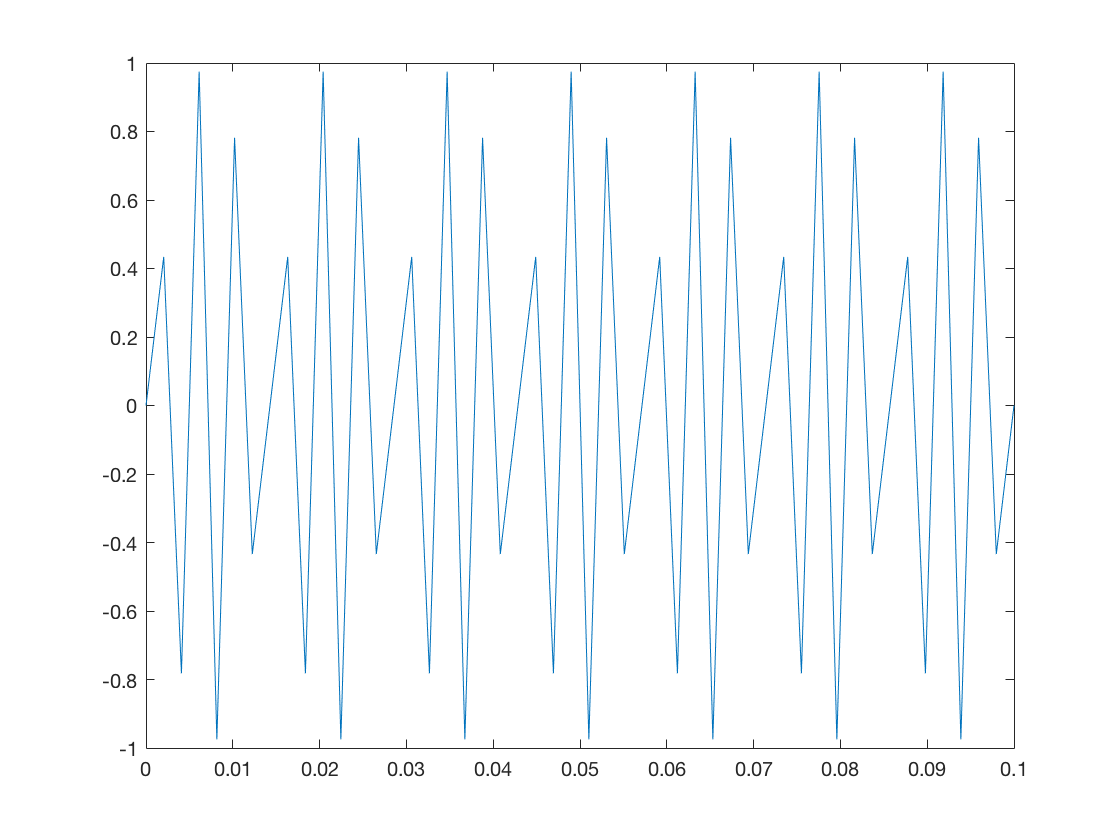
\includegraphics[scale=0.25]{plot1.png}
    \caption{plot1}
    \label{fig:plot1}
\end{figure}

\begin{figure}[h!]
    \centering
    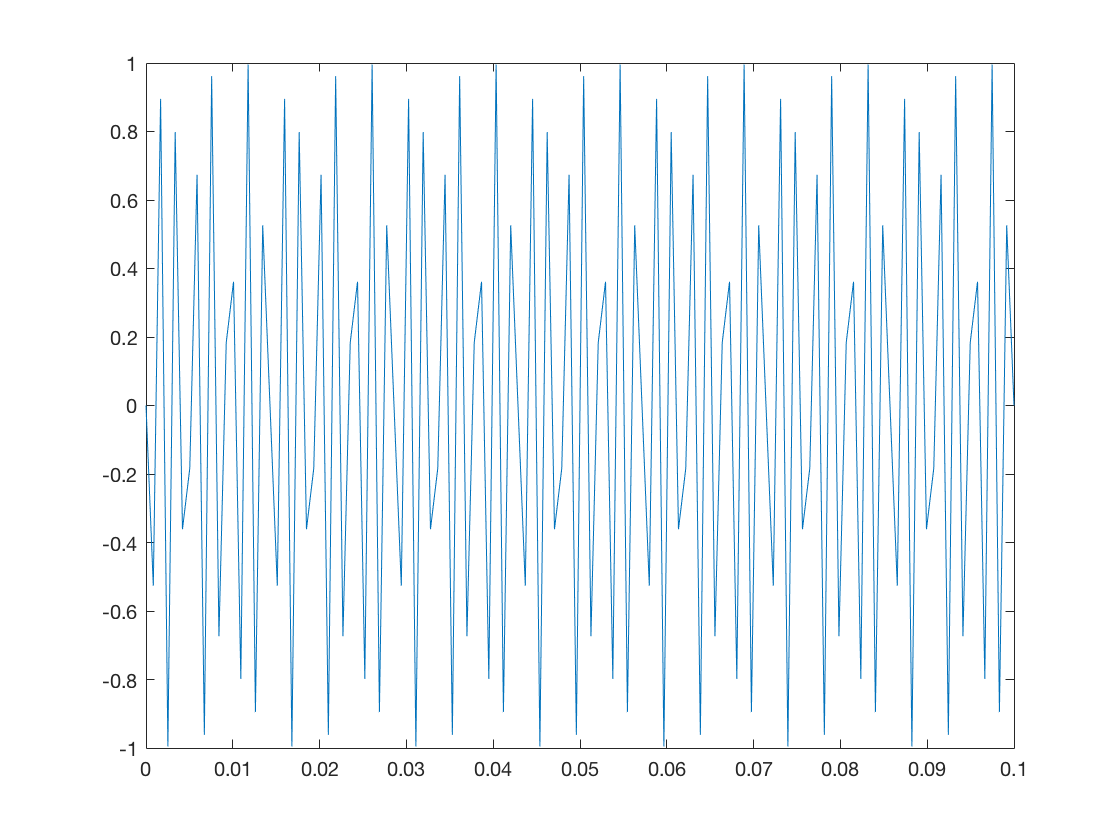
\includegraphics[scale=0.25]{plot2.png}
    \caption{plot2}
    \label{fig:plot2}
\end{figure}

\begin{figure}[h!]
    \centering
    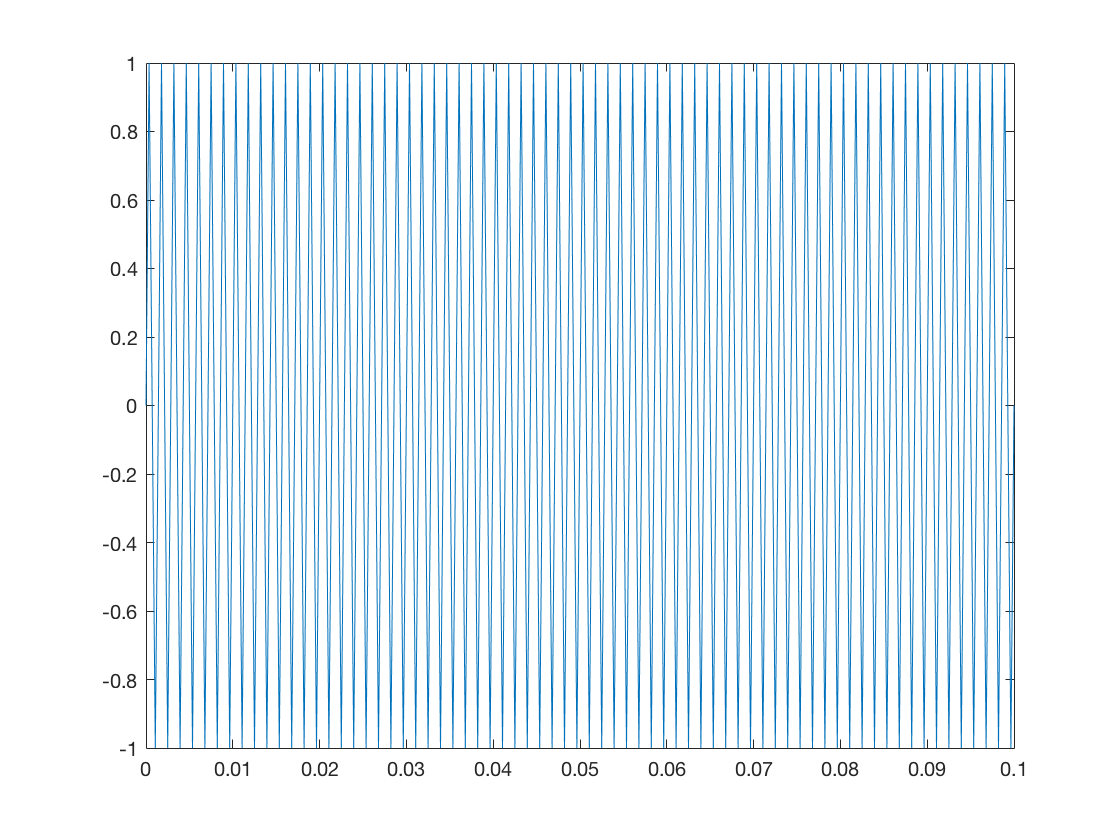
\includegraphics[scale=0.25]{plot3.png}
    \caption{plot3}
    \label{fig:plot3}
\end{figure}
\newpage

\subsubsection{assignment 3}
RESULTAT FRA OPPG 6.03
\begin{figure}[h!]
    \centering
    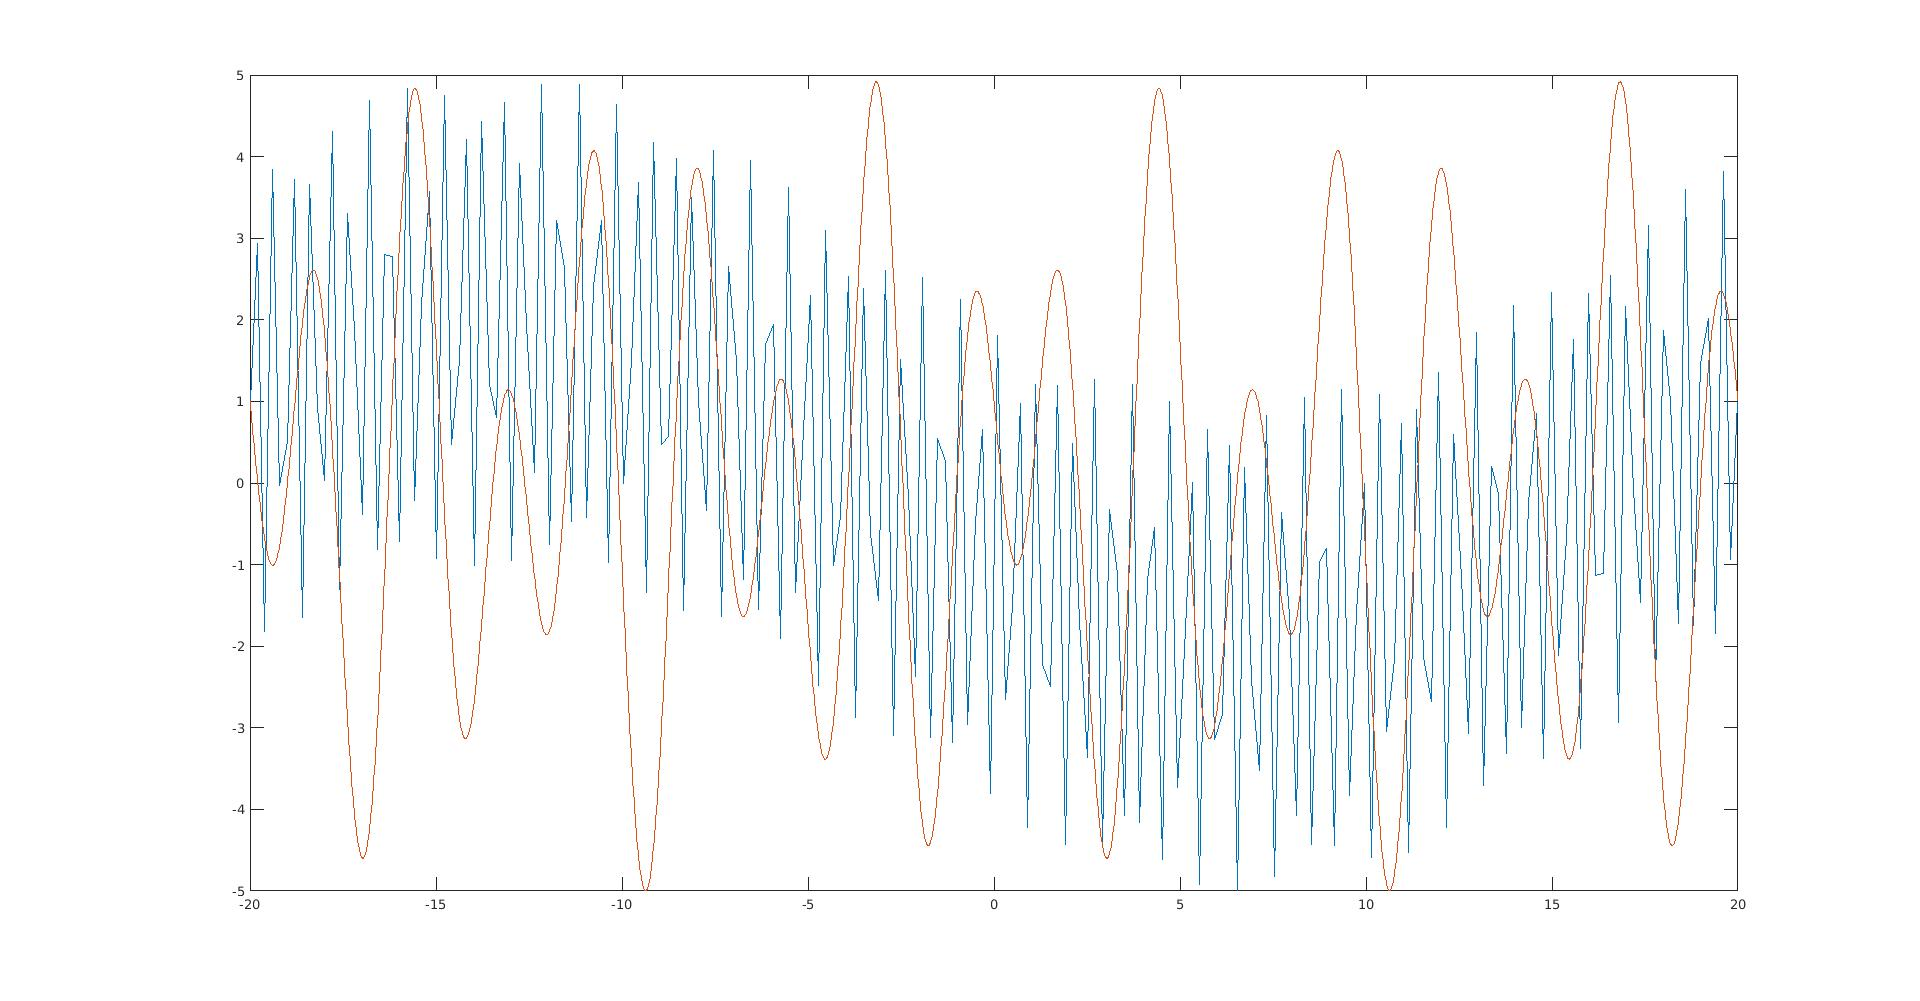
\includegraphics[scale=0.15]{OPPG63.jpg}
    \caption{plot1}
    \label{fig:plot1}
\end{figure}

\begin{figure}[h!]
    \centering
    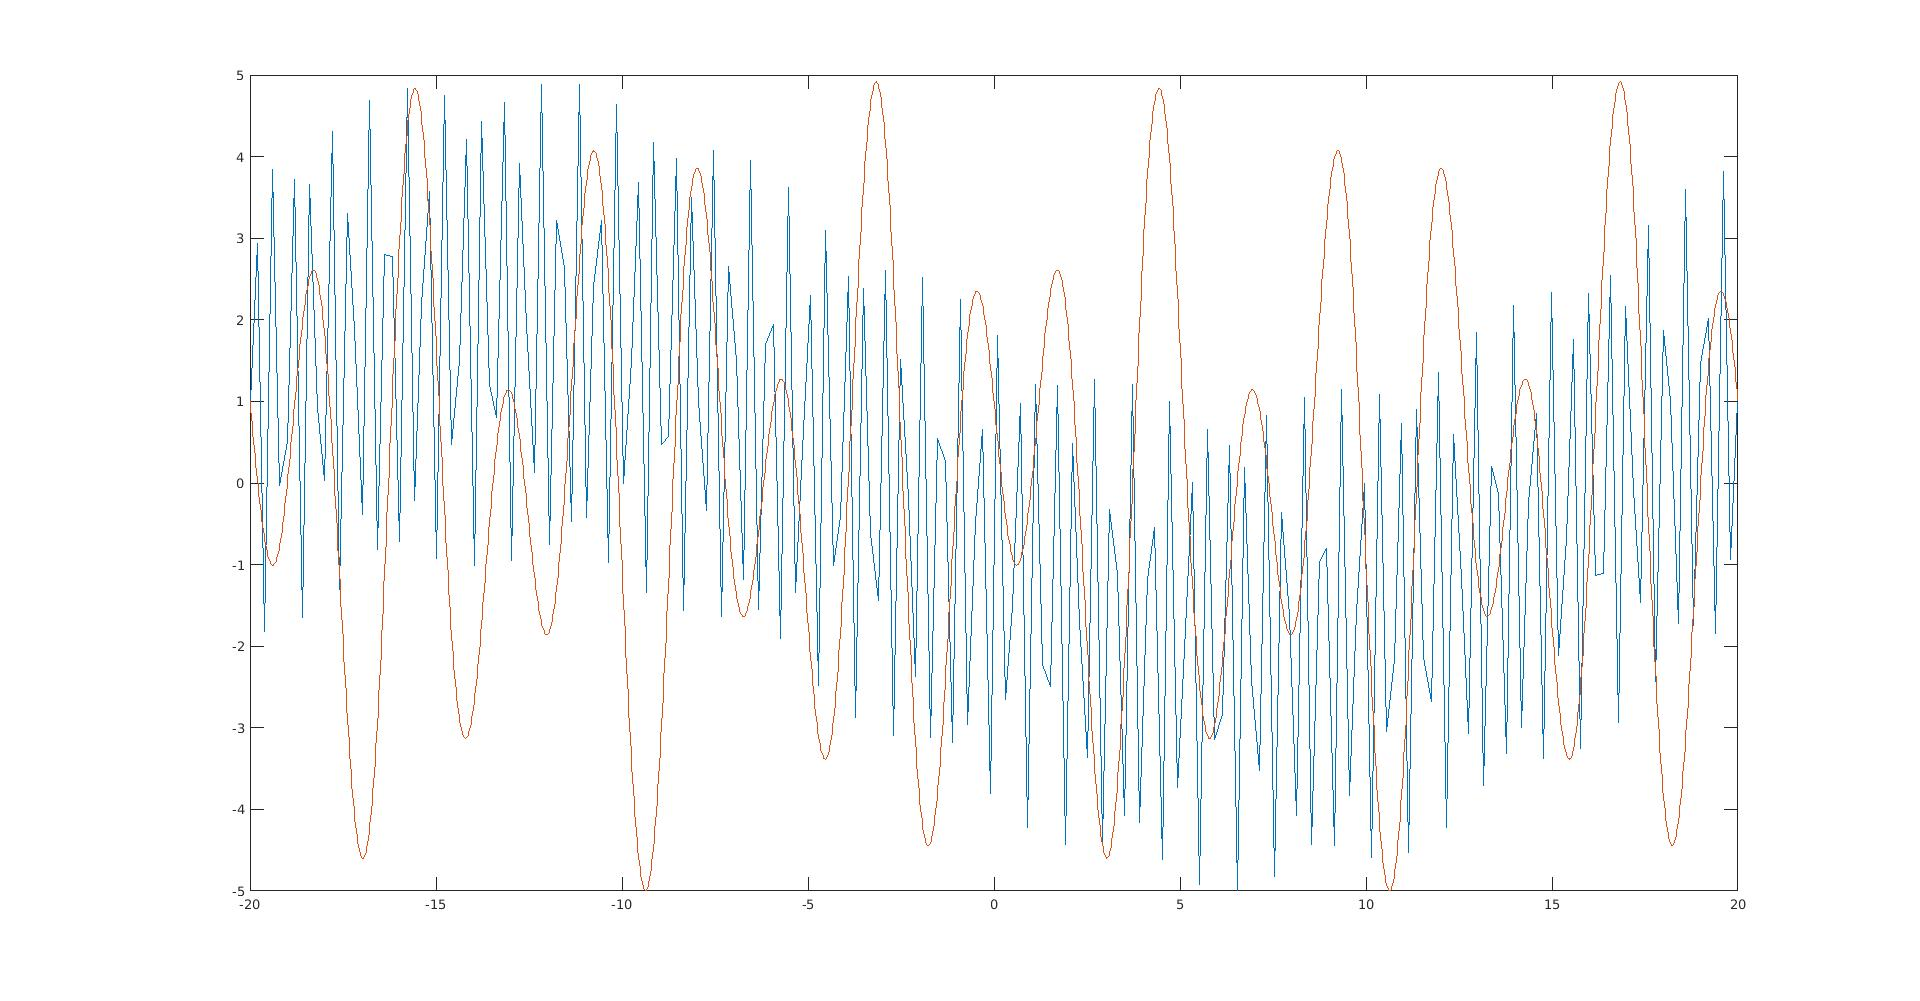
\includegraphics[scale=0.15]{OPPG63_1.jpg}
    \caption{plot2}
    \label{fig:plot2}
\end{figure}

\begin{figure}[h!]
    \centering
    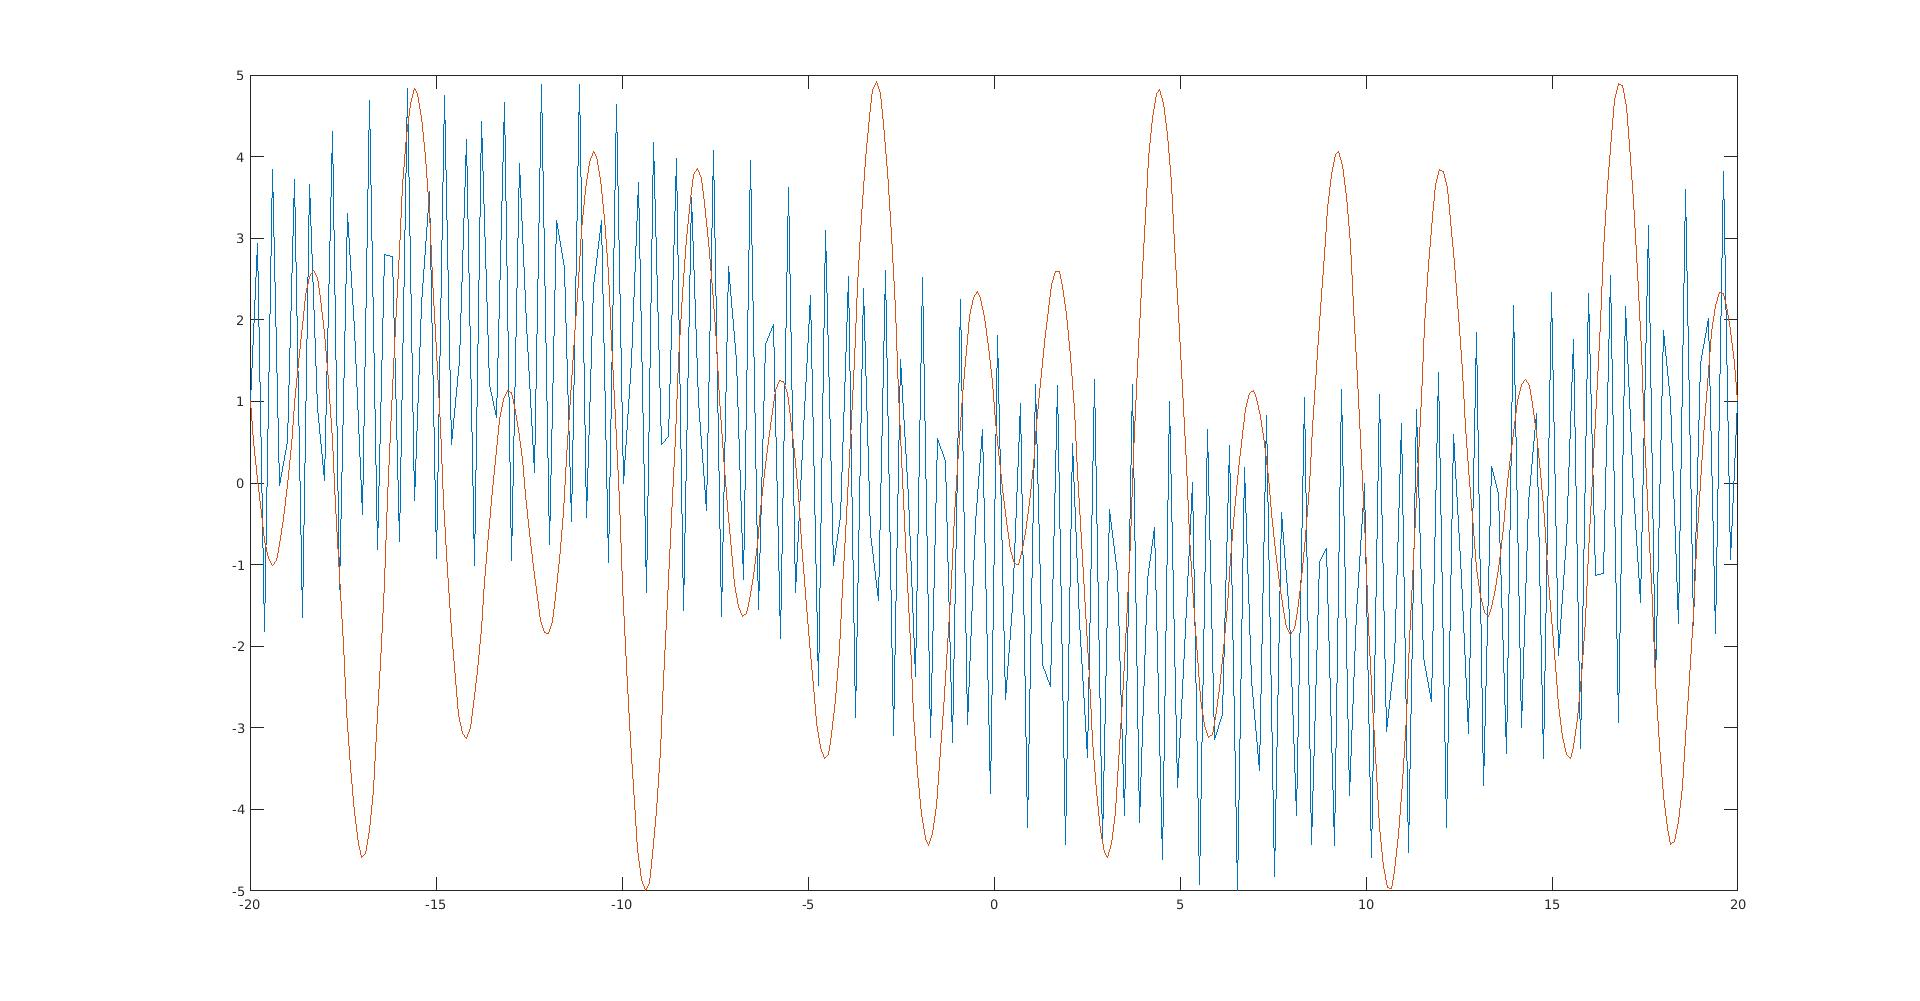
\includegraphics[scale=0.15]{OPPG63_2.jpg}
    \caption{plot3}
    \label{fig:plot3}
\end{figure}

\newpage
\subsubsection{assignment 6.17}
RESULTAT FRA OPPG 6.17
\begin{figure}[h!]
    \centering
    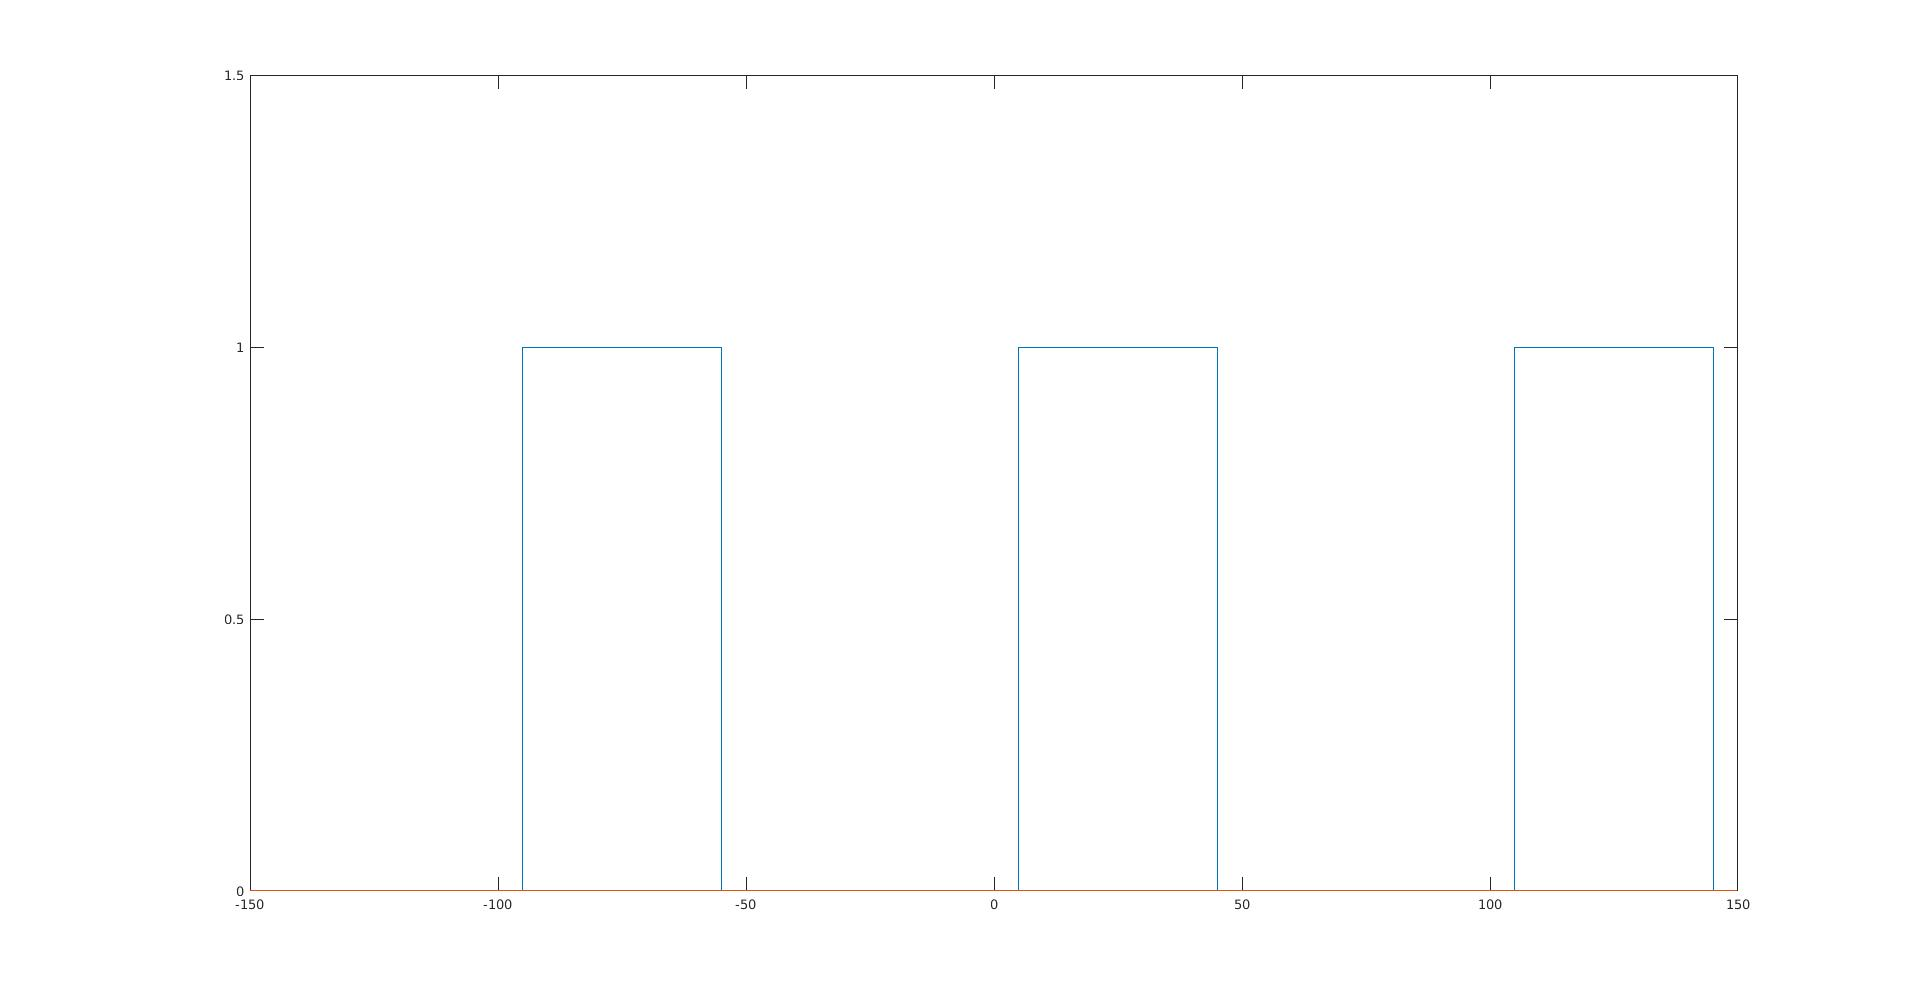
\includegraphics[scale=0.15]{OPPG617.jpg}
    \caption{plot1}
    \label{fig:plot1}
\end{figure}


\end{document}